%! Author = User
%! Date = 25/12/2020

% Preamble
\documentclass[a4paper, amsfonts, amssymb, amsmath, reprint, showkeys, nofootinbib, twoside]{revtex4-2}

% Packages
\usepackage{amsmath}
\usepackage[english]{babel}
\usepackage[utf8]{inputenc}
\usepackage{amssymb}
\usepackage{float}
\usepackage[labelformat=simple, labelsep=colon]{subcaption}
\DeclareCaptionSubType*{figure}
\renewcommand\thesubfigure{Fig.~\thefigure\alph{subfigure}}
\usepackage{graphicx}
\usepackage{import}


% Document
\begin{document}
    \title{Casting A light on the shape of a DNA molecule}
    \author{Alon Levi}
    \affiliation{The Hebrew University of Jerusalem}
    \author{Edo Mor}
    \affiliation{The Hebrew University of Jerusalem}
    \date{\today}
    \begin{abstract}
        In this work we study interference phenomena in the visible spectrum using a camera and a diffracting body.
        We show that the shape of a helix can be reconstructed using 1-D sections of its' diffraction pattern on the the far field approximation.
    \end{abstract}
    \maketitle

    \section{Introduction}\label{sec:introduction}
The structure of small-scale objects, such as a DNA molecule, is important to know, in order to understand many of their features.
The main challenge in measuring those characteristics is that some of them are too small for the equipment we currently have to detect.
One method used to overcome this obstacle is light diffraction and the unique patterns it creates when encountering such objects.
In this article we'll demonstrate some of the main features of light diffraction and how they can be used to infer the shape and size of 2-D objects, we will focus on a helix.
The helix will approximate the DNA molecule which is essentially a double helix and whose diffraction pattern can be seen in Figure~\ref{fig:Single double DNA}.
\begin{figure}[H]
    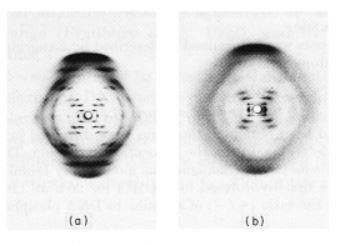
\includegraphics[width=1\columnwidth]{figures/DNA diffraction.PNG}
    \caption{Diffraction patterns of DNA complexes}
    \label{fig:DNA diffraction}
\end{figure}





    \section{Theoretical background }
The nature of flight is a much discussed topic
One view on the matter is that light behaves like a wave as can be seen by the maxwell equations,
one possible solution to the maxwell equations in vacuum is $\vec{E}=\frac{\vec{E_0}}{2}e^{i \left( \vec{k}\cdot\vec{r}-\omega t \right)}+c.c$
and $\vec{B}=\frac{\vec{B_0}}{2}e^{i\left( \vec{k}\cdot\vec{r}-\omega t \right)}+c.c$ where $\|\vec{B_0}\|=\frac{\|\vec{E_0}\|}{c}$ and $\vec{B_0}\bot\vec{E_0}$
which describes a plane wave propagating in the $\vec{k}$ direction.\\
Under this interpretation we expect light to Create an interference pattern when propagating passed a block.\\
The Huygens principle states that each point in a wavefront can be treated as a point wave source,
To define the shape we shall use an optical transference function (\textbf{OTF}) $T(x,y)$
defined to be 1 where the light is completely unobstructed 0 where no light passes threw and can get any complex value depending on the properties of the block
let us also omit the $+c.c$ from now on.\\
For convenience we shall call the axis perpendicular to our block $z$ and the axis in its plane $x$ and $y$ furthermore we shall call the plane where our wave meets the block
the $z=0$ plane, Thus the wave immediately after the block is expressed by $U_o(x,y,0^-)T(x,y)e^{-i\omega t}$ Where $U_o(x,y,z)$ In the spatial part of the wave function
describing the origin illuminating our block.
We shall mark $\psi(x,y,0,t)=T(x,y)U_o(x,y,0^-)e^{-i\omega t}$ As the wavefunction describing our wave immediately after the block
Such a wavefunction can be described in terms of plane waves as $\psi(\vec{r},t)=\left( \frac{1}{\sqrt{2\pi}} \right)^3 \iiint\limits_{-\infty}^{\infty}b(\vec{k})e^{i \left( \vec{k}\cdot\vec{r}-\omega_k t \right)}d^{3}k$
where $\omega_k=\|\vec{k}\|c=k_{0}c \Rightarrow k_z=\sqrt{k_0^2-k_x^2-k_y^2}$
\\Let us now examine the interference pattern created by a plain wave When hitting a block of some shape.\\

    \section{Experimental methods and apparatus}\label{sec:experimental-technique-and-apparatus}
To examine the diffraction pattern from different slit patterns (and eventually a helix) we use the system described in Figure~\ref{fig:Apparatus}.
\begin{figure}[H]
    \centering
    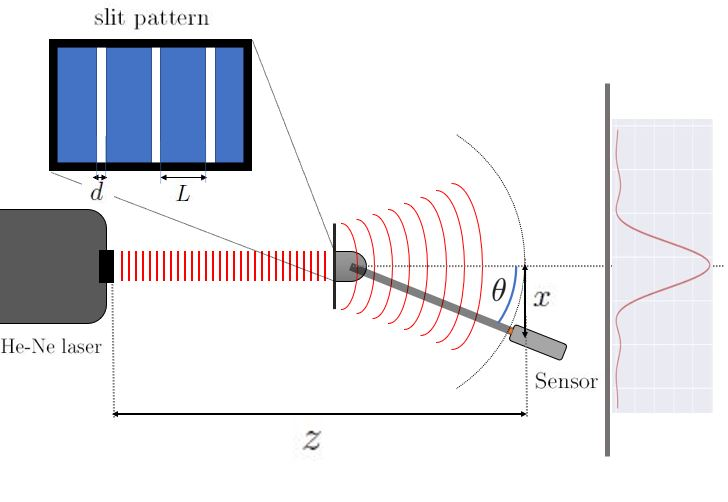
\includegraphics[width=0.9\columnwidth]{figures/Apparatus.JPG}
    \caption{A description of the system used to measure the intensity of light coming from a He-Ne laser at different angles. An example of a slit
    pattern is shown, but can be swapped for any diffracting object}
    \label{fig:Apparatus}
\end{figure}
Where the He-Ne laser produces an approximately monochromatic plane wave with $\lambda=632.8 [nm]$ and our sensor is at a fixed distance from the slits with $z=0.855 [m]$.
The angle $\theta$ and the Intensity $I$ were measured using a resistor and a photodiod, the voltage on these resistors ($V\propto\theta,I$) was
measured as a function of time.
Prior to every measurement we align the laser beam with the sensor by detecting the point of maximum intensity, then place the slits perpendicular to
the beam.
This procedure is key to make sure our plain wave is reaching the slits with uniform phase and avoid major changes to our expected diffraction pattern.
The sensor was then moved to scan the intensities at some range of angles which were then converted to distances on our theoretical screen. We also
note that the sensor has an iris through which the light goes before measured, thus all light within that width is accounted for when measuring a
certain angle.
Our expected intensity is then $I(x)=\int\limits_{x-d}^{x+d}I(x')dx'$.
For the helix we use a similar set up, removing the sensor and replacing the slit pattern with the helix.
The measurement was then taken with a camera and the photo was compared to a numeric model.
    \section{Results}\label{sec:results}
According to equation \eqref{eq:farfield} and the specified approximations the interference pattern can be calculated using
the 2 dimensional fourier transform of the shape of the slit, Taking the inverse fourier transform of the pattern should result
In the square of the shape of the slit (since when calculating the intensity the square of $U$ was taken)
as can be shown by Fig.\ref{fig:expansion theory measurements}
\begin{figure}[H]
    \centering
    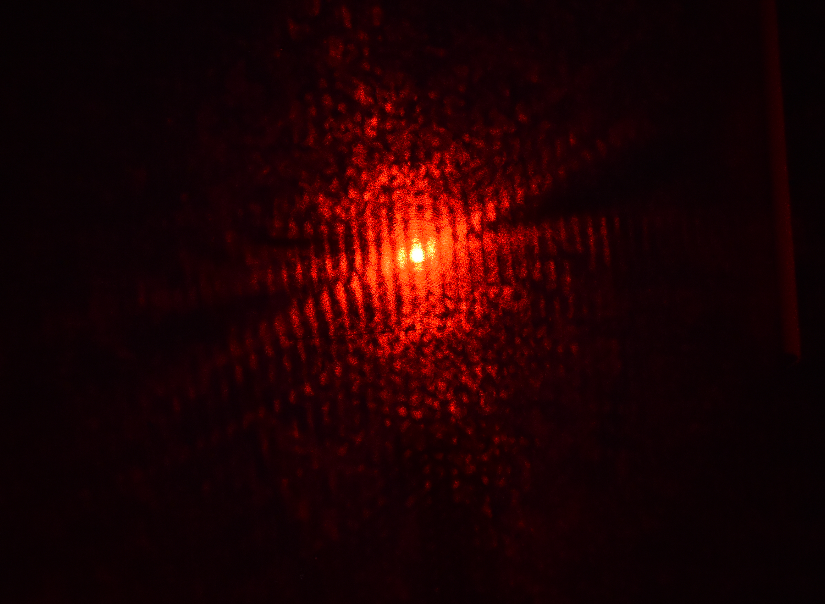
\includegraphics[width=0.9\columnwidth]{figures/expantion meshured interferemce.png}
    \caption{interference pattern measured as a result of diffraction with a helix}
    \label{fig:expansion measured interference pattern}
\end{figure}
\begin{figure}[H]
    \centering
    \begin{subfigure}{0.48\columnwidth}
        \centering
        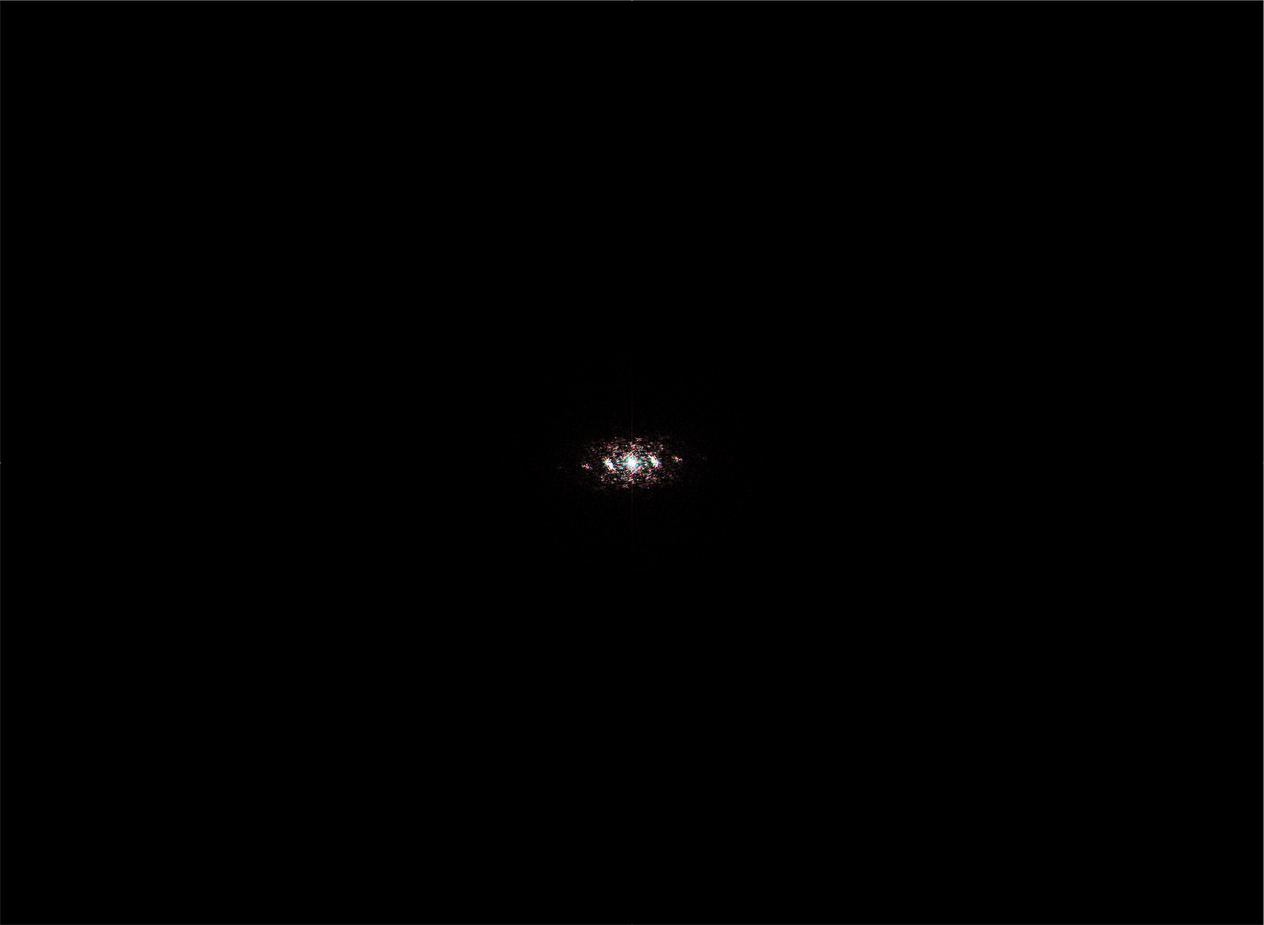
\includegraphics[width=0.9\columnwidth]{figures/expantion fourie transform.png}
        \caption{inverse discrete fourie transform calculated from the interference pattern at of the helix }
        \label{fig:expansion inverse fourie transform measured}
    \end{subfigure}\hfill
    \begin{subfigure}{0.48\columnwidth}
        \centering
        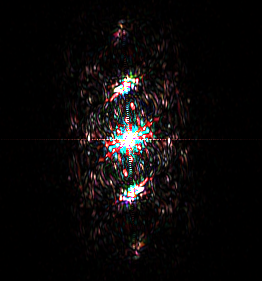
\includegraphics[width=\columnwidth]{figures/expantion fourie transform magnified.png} % second figure itself
        \caption{magnification of\ref{fig:expansion inverse fourie transform measured}}
        \label{fig:expansion fourie transform magnified}
    \end{subfigure}

    \label{fig:expansion theory measurements}
\end{figure}

While far from identical, the two images have some similarities, the bright section in the middle of the "squared helix" and the darker rings around it.
To be able to further analyse the diffraction pattern of a helix let us deconstruct it into segments.
Slit patterns can be thought of as an approximation of one-dimensional sections of a helix, they also have a well-known solution which we have confirmed by measuring the diffractions from those slit patterns.

\begin{figure}[H]
    \centering
    \begin{subfigure}{0.48\columnwidth}
        \centering
        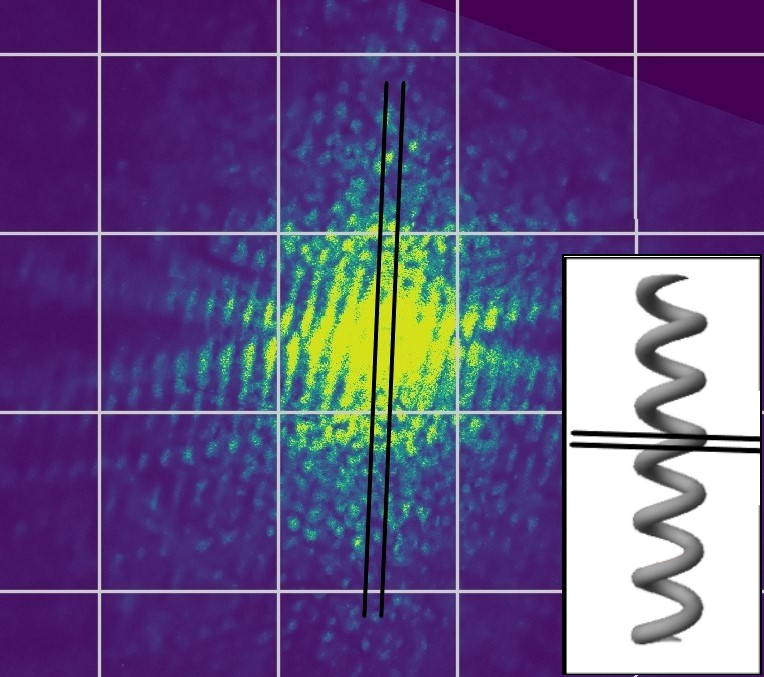
\includegraphics[width=\columnwidth]{figures/HelixSection2.png} % second figure itself
        \caption{Single slit section}
        \label{fig:HelixSection1}
    \end{subfigure}
    \begin{subfigure}{0.48\columnwidth}
        \centering
        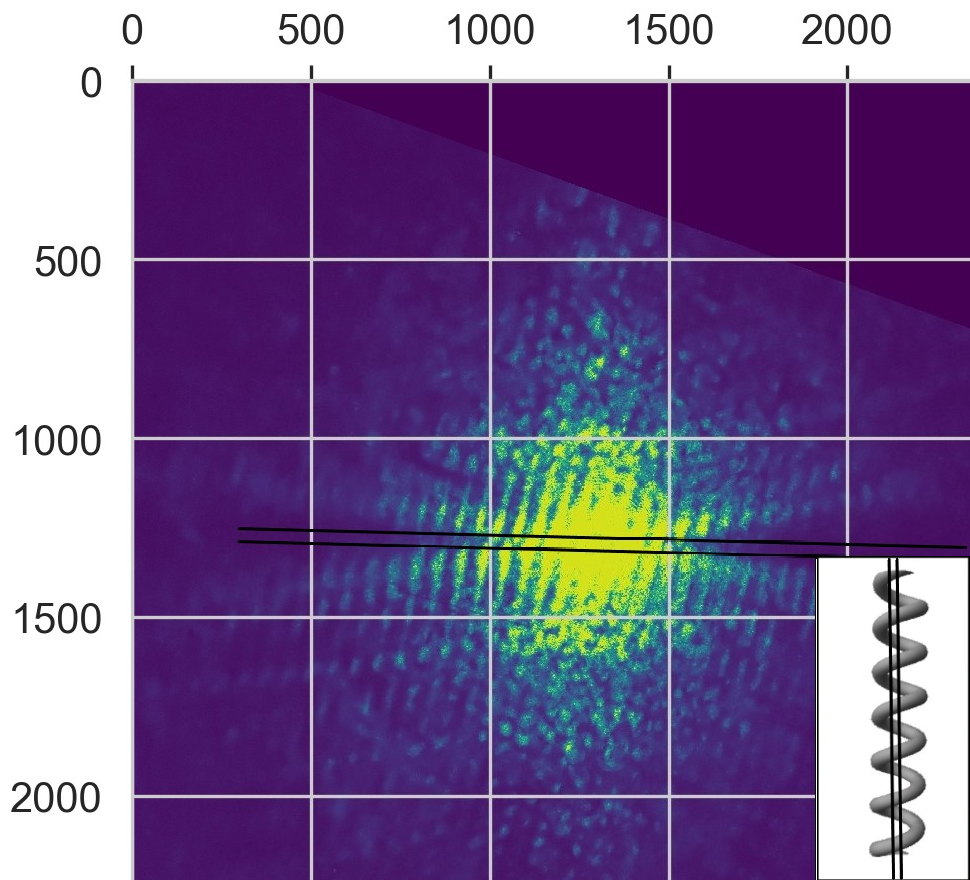
\includegraphics[width=\columnwidth]{figures/HelixSection1.png}
        \caption{N-slits section}
        \label{fig:HelixSection2}
    \end{subfigure}
    \begin{subfigure}{0.46\columnwidth}
        \centering
        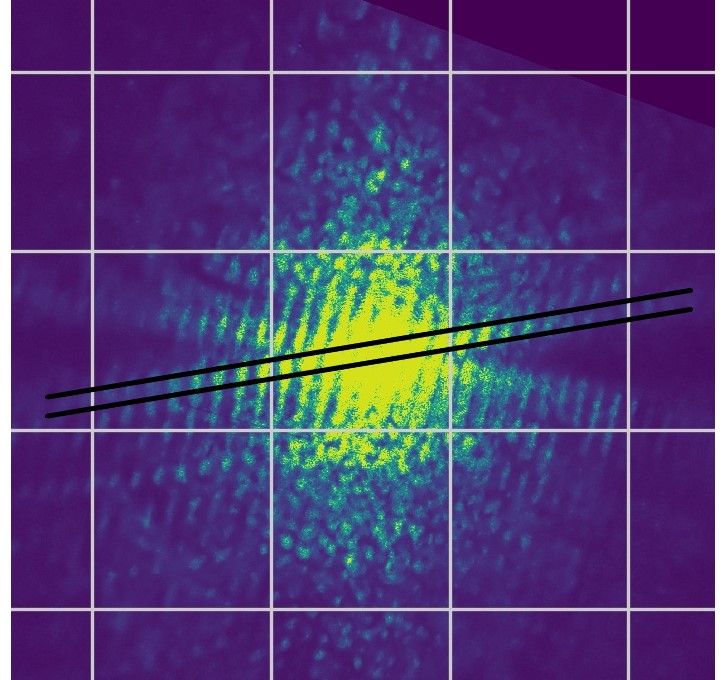
\includegraphics[width=\columnwidth]{figures/HelixSection4.jpg} % second figure itself
        \caption{"X" section 1}
        \label{fig:HelixSection3}
    \end{subfigure}
    \begin{subfigure}{0.48\columnwidth}
        \centering
        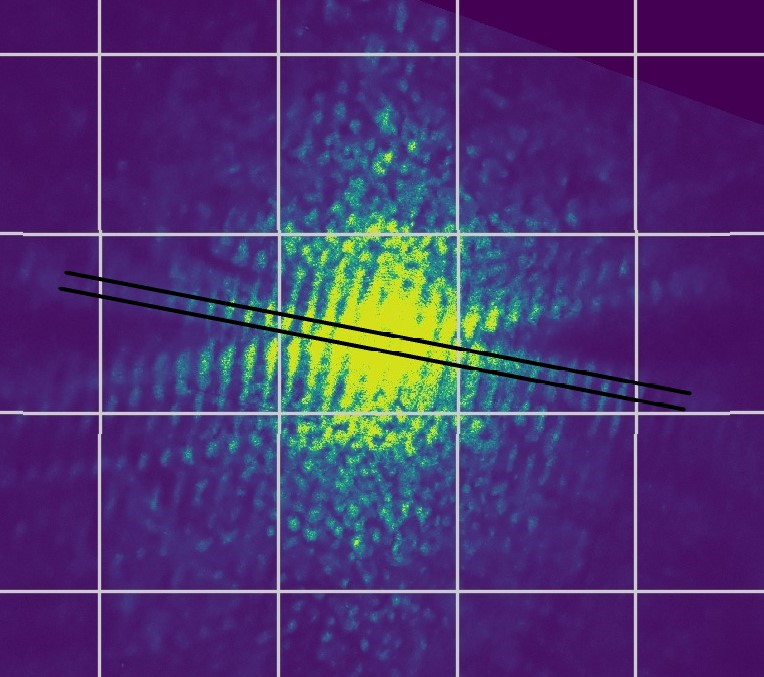
\includegraphics[width=\columnwidth]{figures/HelixSection3.jpg} % second figure itself
        \caption{"X" section 2}
        \label{fig:HelixSection4}
    \end{subfigure}
    \caption{Deconstruction of diffraction pattern to known 1D sections.}
    \label{fig:HelixSections}
\end{figure}

\subsection{Single slit section}
Taking the horizontal section of the helix we noticed that it can be described as:
\[T(x)\approx 1-rect\left(\frac{x}{2R}\right)\]
Where we treat the helix as approximately a cylinder, which is, in the context of our 1-D section (\ref{fig:HelixSection1}), the complement diffracting body of a single slit.
\begin{figure}[H]
    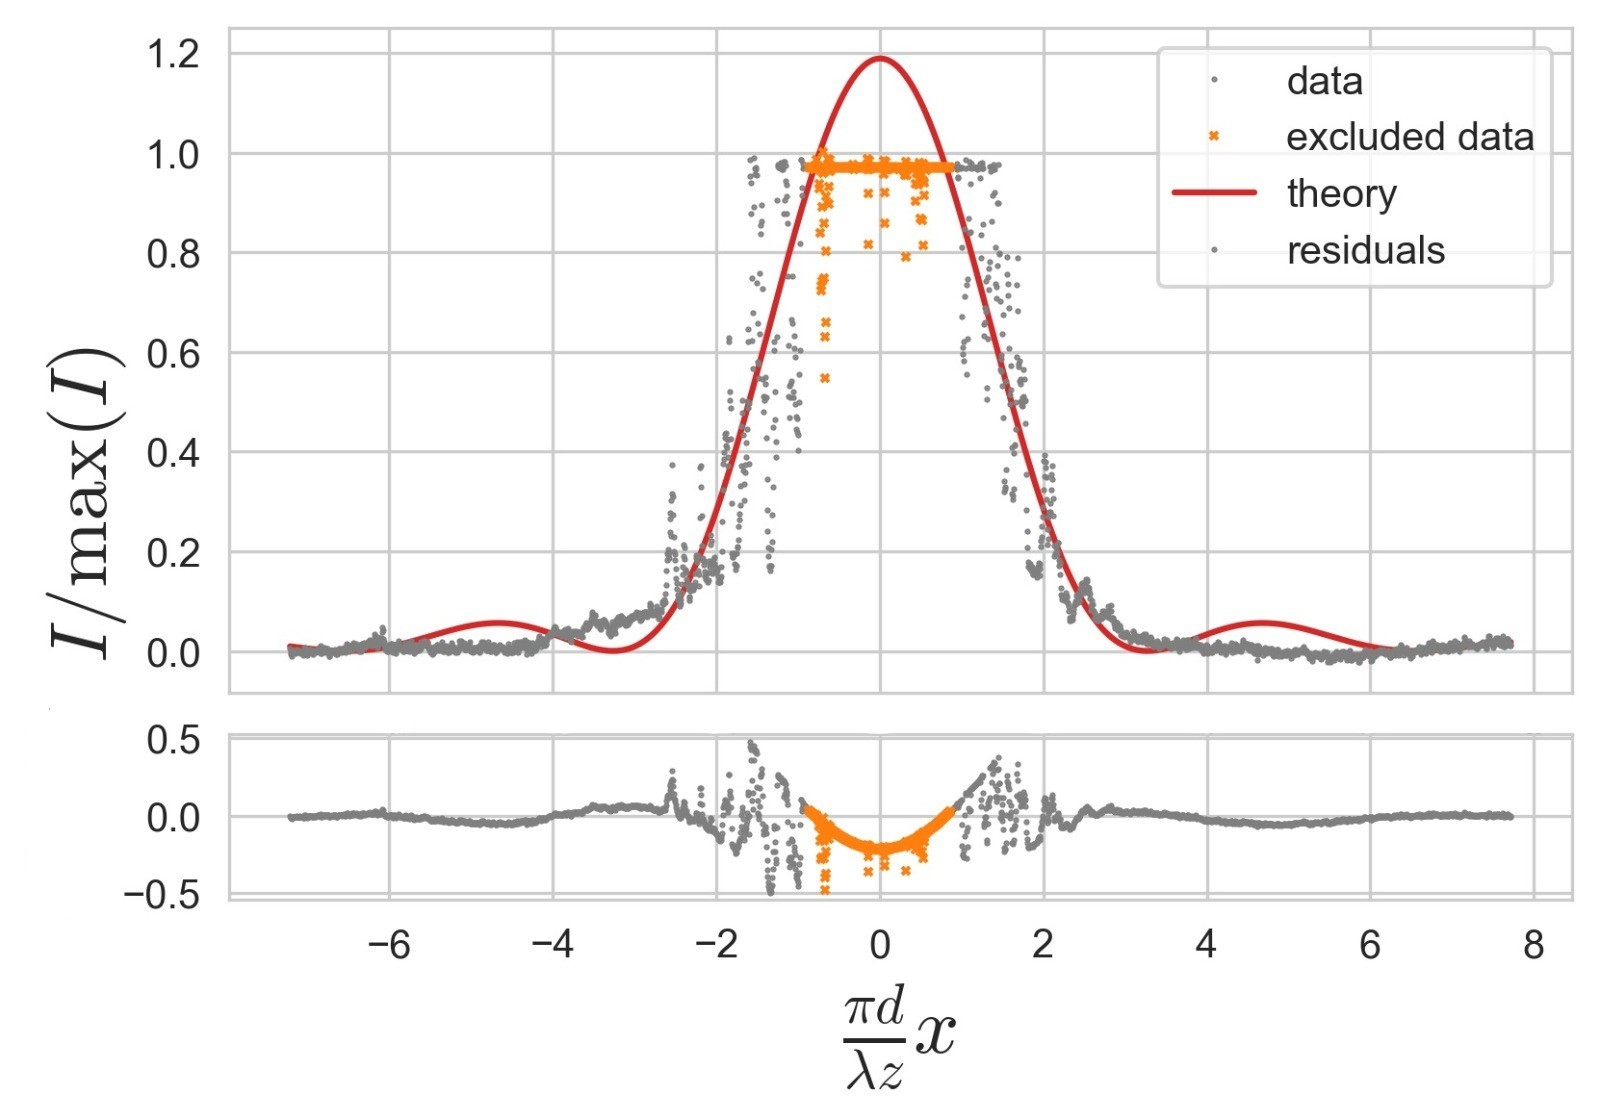
\includegraphics[width=0.9\columnwidth]{figures/Single slit section.jpeg}
    \caption{A fit for the single slit section of the helix using our model for single slit diffraction}
    \label{fig:Single slit section}
\end{figure}
The single slit model used in Figure~\ref{fig:Single slit section} describes the diffraction of our helix section with an error of $\sigma\approx0.1$.
The camera's sensor was saturated around $x=0$ and therefore that data was excluded from the fit.
We can also see oscillations around the main peak of the fit that increase in amplitude closer to $x=0$, we believe those are the result of the lack of focus in our picture.
There are oscillations in intensity along the "X" sections and the closer we get to the center of the single slit section the more they affect the intensity we measure.
\\
The radius of the helix according to the fit:
\[\]

\subsection{N slits section}
If we take the section perpendicular to that we've discussed earlier, there's a resemblance to the n slits pattern.
The width of the helix is now the distance between two slits, and the pitch is the width of each slit.
For the section taken along the middle of the helix we have: \[L=\frac{p}{2}-d',d'=\frac{d}{\sin \theta}\]
Where $d'$ is the width of the effective slit.
\begin{figure}[H]
    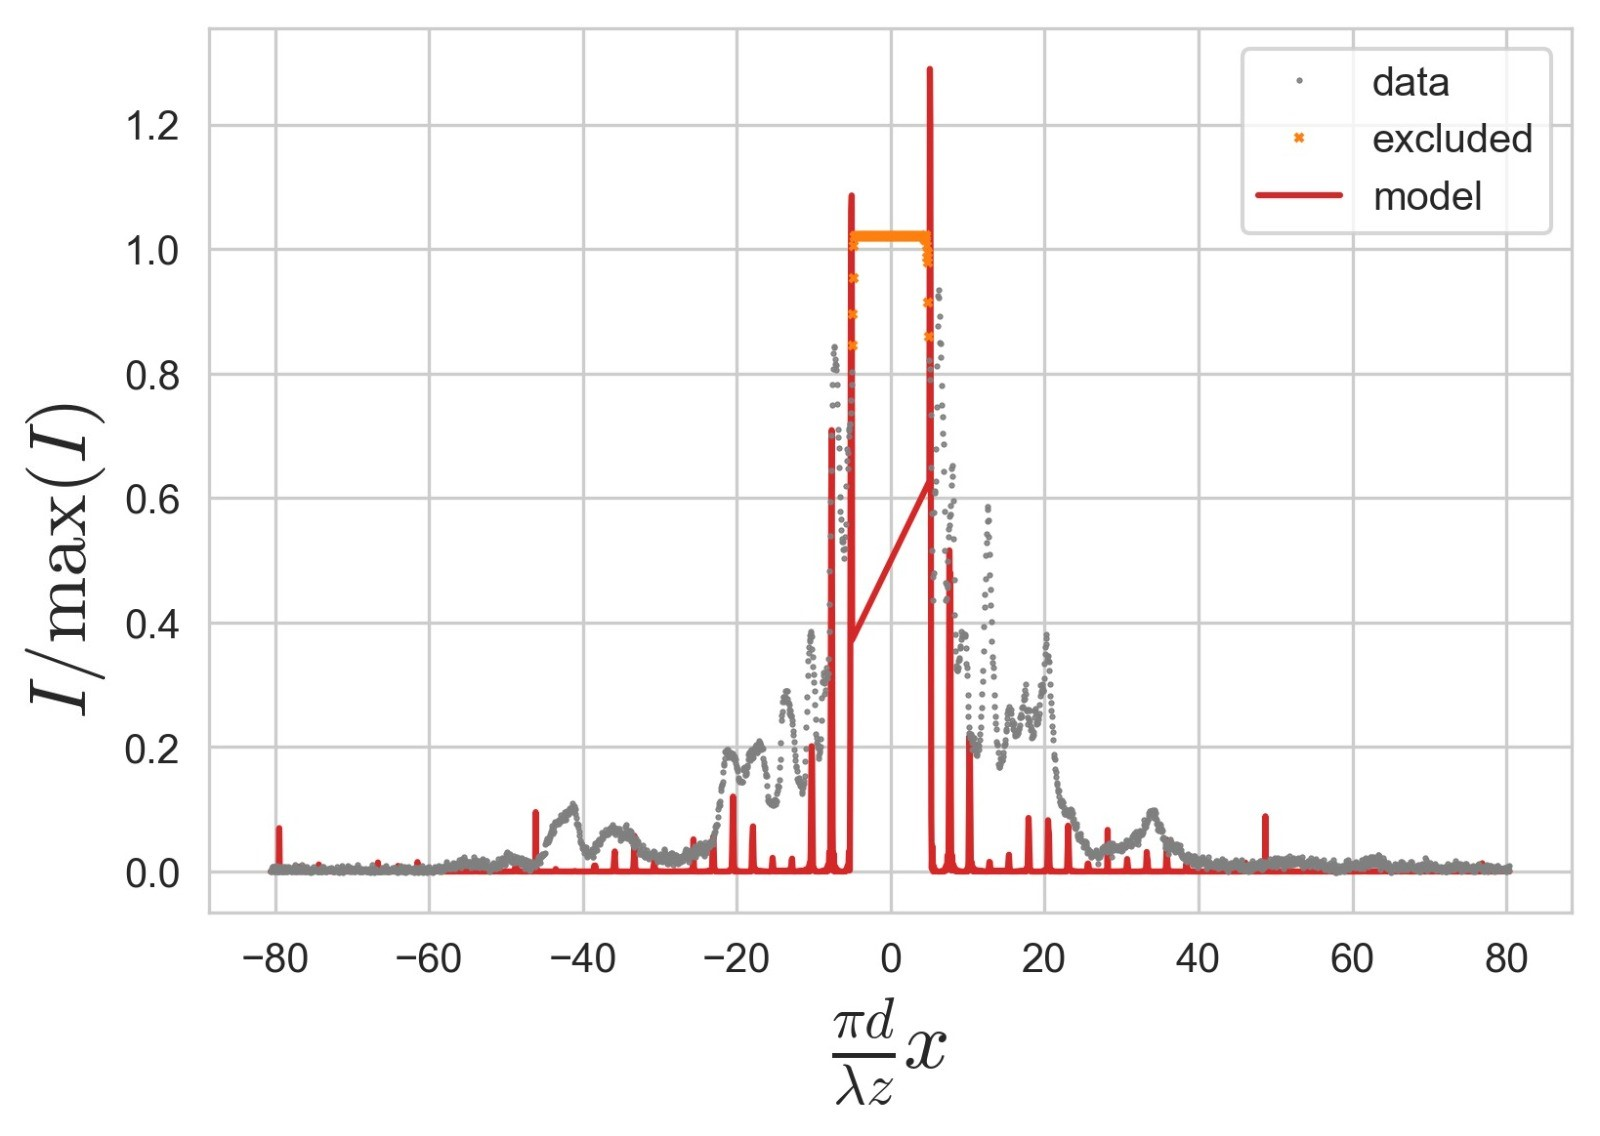
\includegraphics[width=0.9\columnwidth]{figures/n slits section.jpeg}
    \caption{A fit for the N-slits section using our model for N-slits diffraction}
    \label{fig:n slits section}
\end{figure}
Our model for N-slits is far from being able to predict the diffraction along the relevant section, we believe this is due to the focus problem discussed earlier.
While the model predicts some of the locations of local maxima, it fails to predict their amplitude and the behaviour of the pattern between those maxima.
The intensity changes faster relative to the single slit model and the focus effect is more dominant for this section.
We therefore decided not to rely on the parameters of the spring extrapolated from the fit.

\subsection{The "X" sections}
The two final sections are another way for us to compute the parameters of the slits.
In the example of N-slits section we saw that the locations of local maxima wasn't extremely affected by our measuring method.
We assume the same is true for the "X" sections (Fig.\ref{fig:X Sections}) and compute $d$ and $p$:
\[\]
Finally using some trigonometry we can get the following relation:
\[R=\frac{p}{4\tan \theta}+\frac{d}{2}\approx \]
The result is of the same scale as what we got from the fit for the single slit section.

    \section{Discussion}
After examining the helix's diffraction pattern and deconstructing it to more familiar segments we were able to infer some of its' features.
Our error was large due to effects caused mainly by measuring method and we weren't able to completely reconstruct the helix from its diffraction pattern.
We have, however, shown that for a semi-translucent sample with typical size of $\lambda$ a reconstruction of its shape
is possible given that the distance from the screen is large enough the error in such reconstruction is proportional to the
size of the screen and most of the details lost due to the cutoff will effect the outer parameter of the shape.
We  would have continued this experiment by taking multiple pictures of the helix, prioritizing maximizing our focus,
and reconstruct the shape of a helix with higher accuracy.
    \section{Appendix}
our sensor is at a fixed distance from the slits with $z=0.855 [m]$.
The angle $\theta$ and the Intensity $I$ were measured using a resistor and a photodiod, the voltage on these resistors ($V\propto\theta,I$) was
measured at a rate of $40[Hz]$ and a resolution of $\Delta V\approx10^{-3}[V]$.
Prior to every measurement we align the laser beam with the sensor by detecting the point of maximum intensity, then place the slits perpendicular to
the beam.
The slits are then moved along the x axis until we measure maximum amplitude for a single slits and n slits, or between the two maxima for double slit patterns.
These procedures are key to make sure our wave is a good approximation for a plain wave and it is reaching the slits with uniform phase thus avoiding major differences from our models' assumptions.
The sensor was then moved to scan the intensities at some range of angles which were then converted to distances on our theoretical screen.
As can be seen in figure \ref{fig:single slit interference with 0.04mm width} the theory for a single slit fits the data well however there are
secondary effects easily observable in the tails of the data that per our understanding are partially caused by the non-linearity of the
photomultiplier and photoelectric sensor, such effects were not taken into account when formulating our theory
However the adjustment can be easily accomplished.
\begin{figure}[H]
    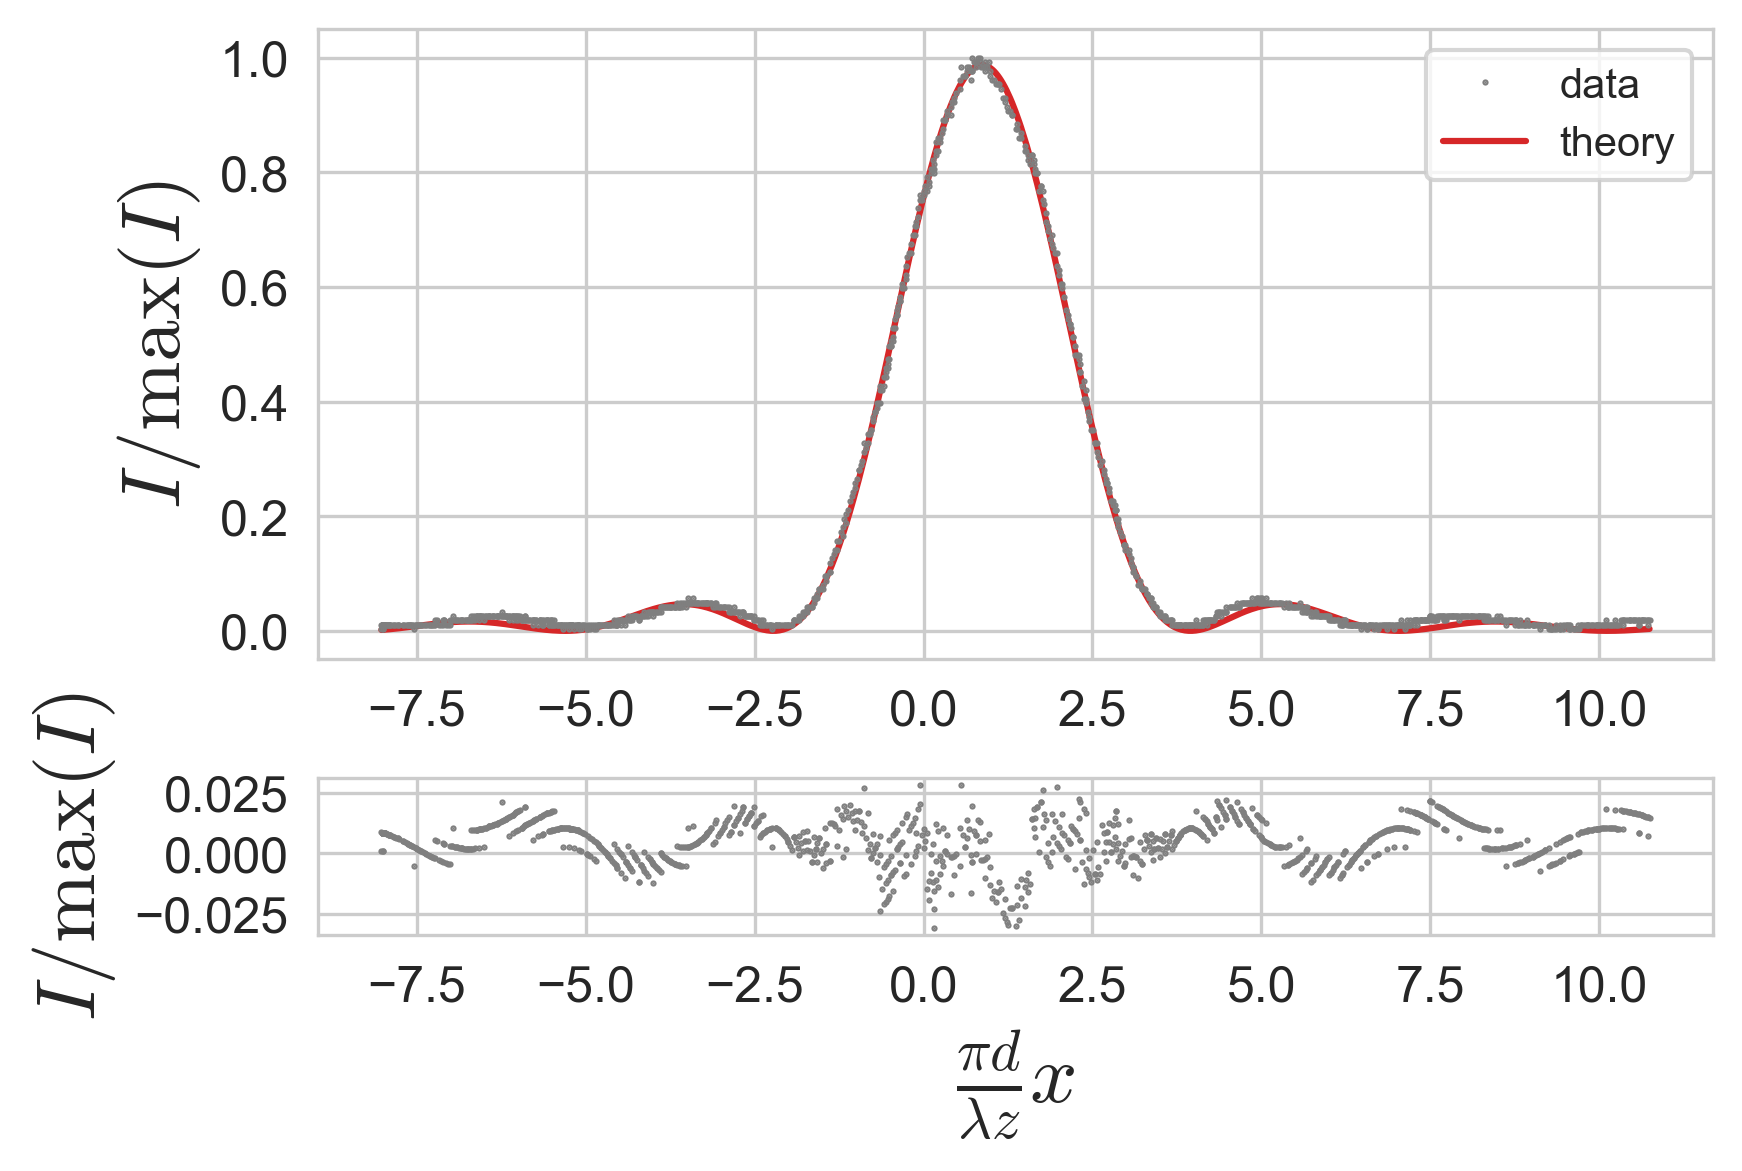
\includegraphics[width=0.9\columnwidth]{figures/single slit interference with 0.04mm width.png}
    \caption{$\lambda$ is the laser wave length $d$ is the width of the slit and $z$ is the distance from the screen}
    \label{fig:single slit interference with 0.04mm width}
\end{figure}
\begin{figure}[H]
	\centering
	\begin{subfigure}{0.5\columnwidth}
		\centering
		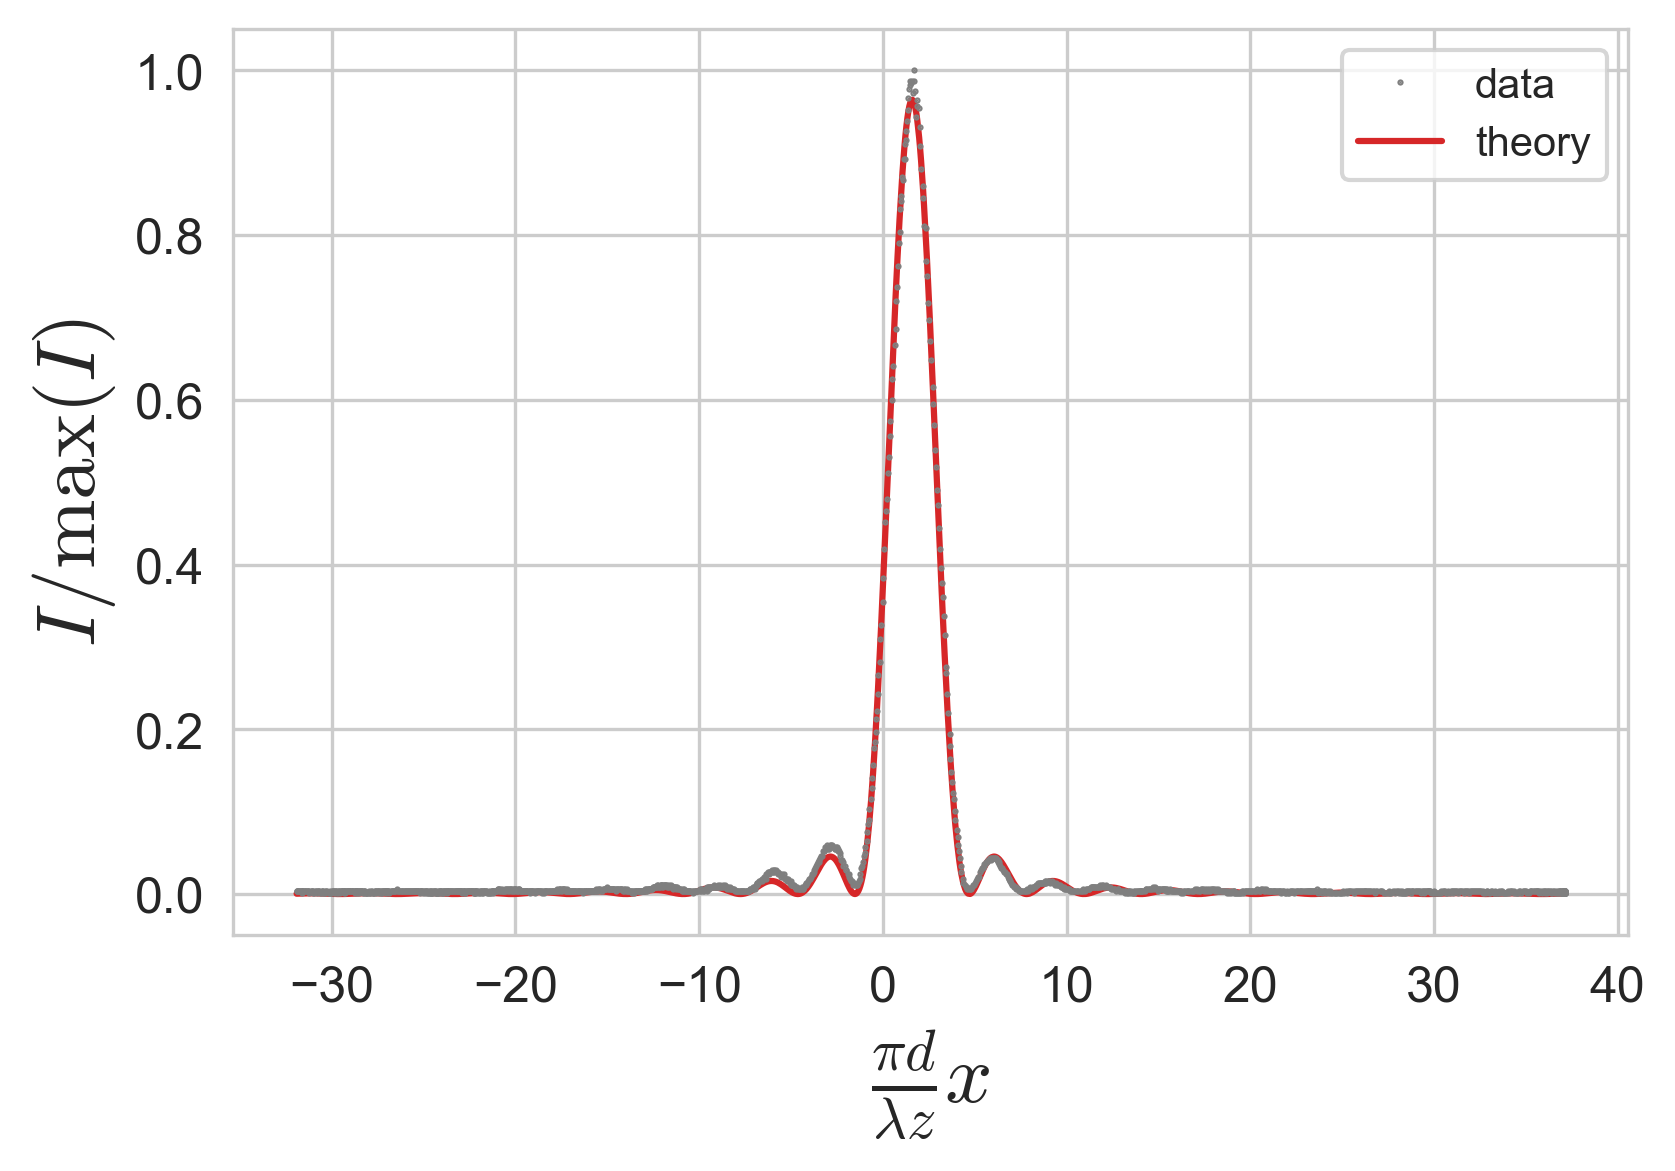
\includegraphics[width=\columnwidth]{figures/single slit interference 0.08mm.png} % first figure itself
		\caption{first figure}
        \label{fig:single slit interference 0.08mm}
	\end{subfigure}\hfill
    \begin{subfigure}{0.5\columnwidth}
        \centering
        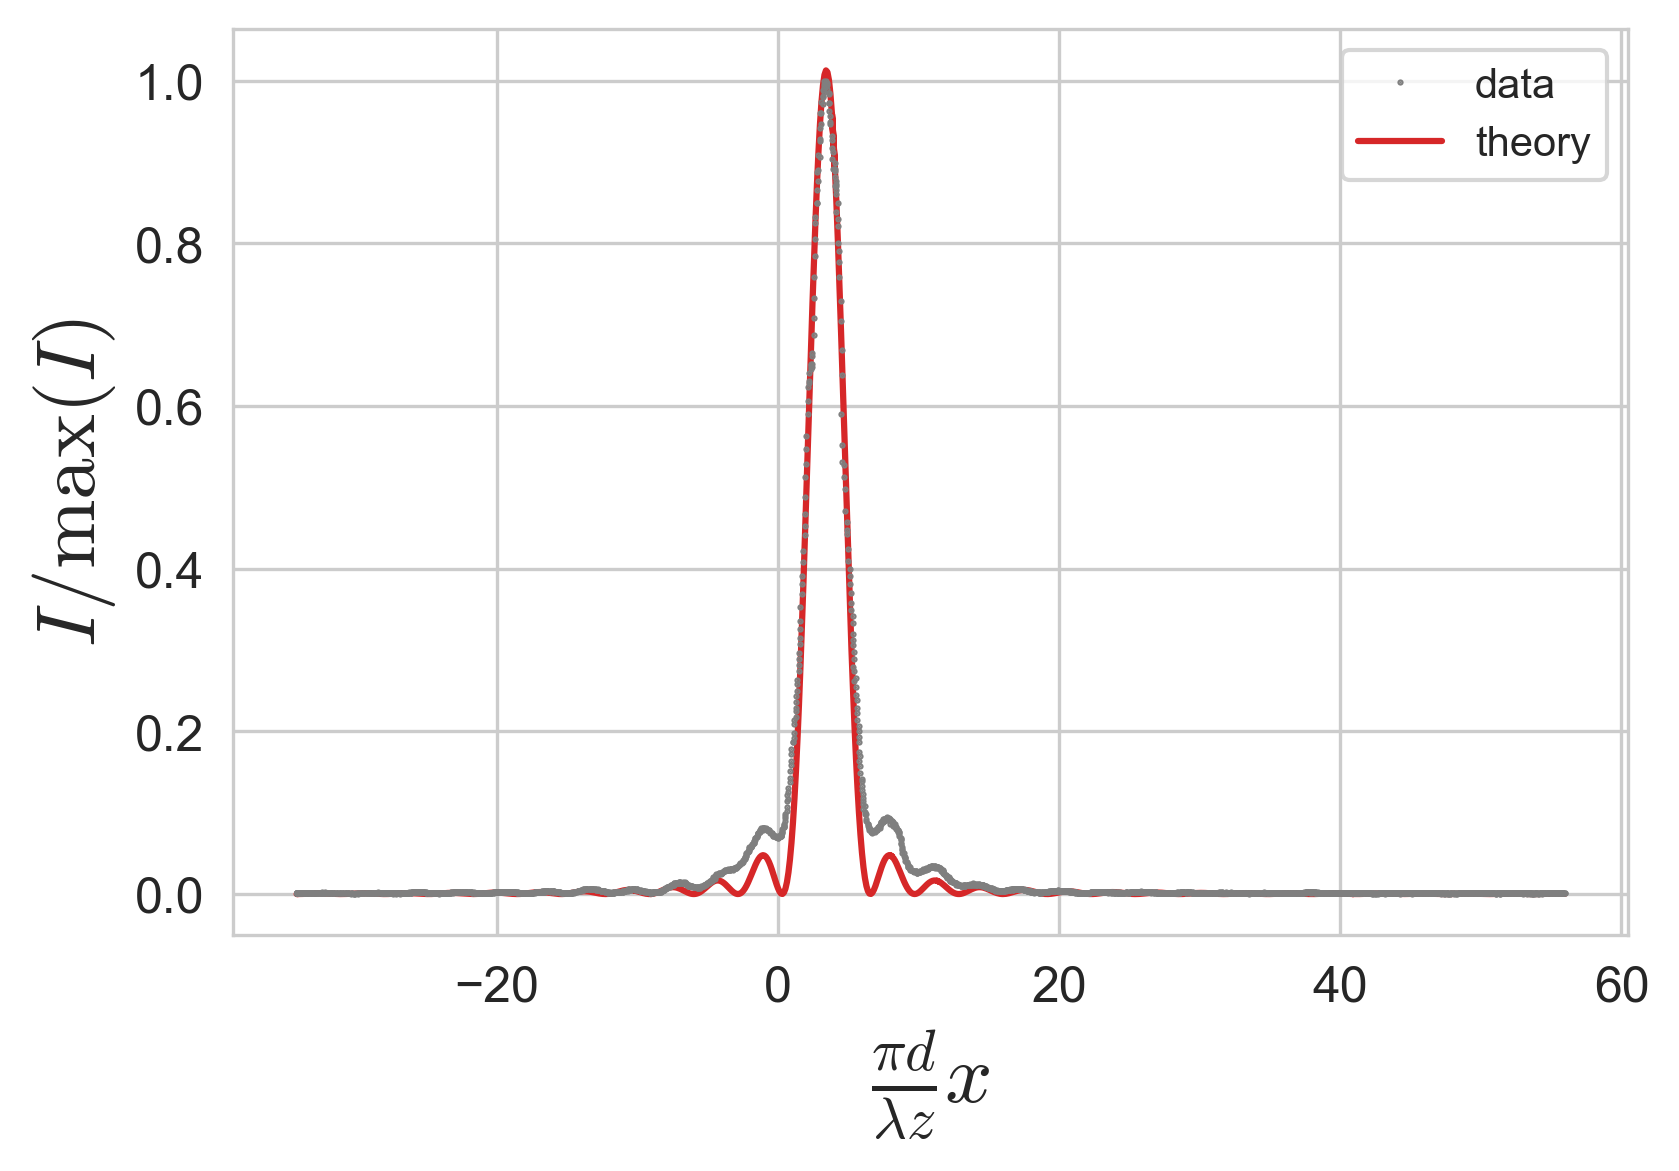
\includegraphics[width=\columnwidth]{figures/single slit interference 0.16mm.png} % second figure itself
        \caption{second figure}
        \label{fig:single slit interference 0.16mm}
    \end{subfigure}
    \label{fig:single slit examples}
\end{figure}



\end{document}